\section{РЕАЛИЗАЦИЯ И АНАЛИЗ ЭФФЕКТИВНОСТИ МОДЕЛЕЙ}

В работе были изучены и реализованы две архитектуры сверточных нейронных сетей: AlexNet \cite{alexnet} и VGGNet \cite{vggnet}.
Были произведены модификации данных моделей под решаемую задачу.
Для реализации использовалась библиотека глубокого обучения \textbf{pytorch}.
Помимо функции потерь оценивалась точность предсказаний.

Для обучения представленных в работе моделей использовался компьютер со следующими характеристиками:
\begin{itemize}
    \item Процессор Intel Core i5 12400h (6 ядер)
    \item 32 ГБ оперативной памяти
    \item Видеокарта AMD Radeon RX6700XT (12 ГБ видеопамяти)
\end{itemize}

\subsection{Предобработка данных}

Исходный датасет состоит из 26179 изображений.
На рисунке \ref{fig:dist} представлена 2D гистограмма распределения разрешения изображений.
\begin{figure}[h]
    \centering
    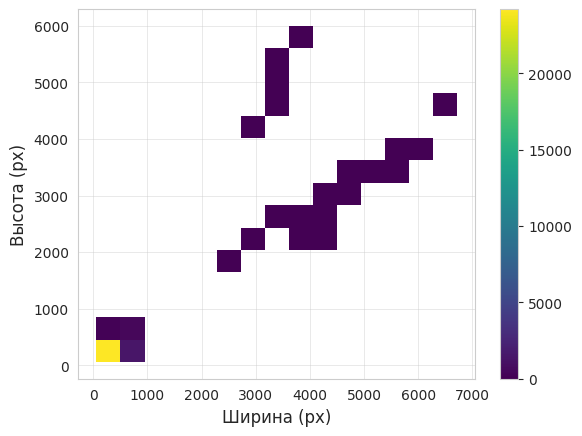
\includegraphics[width=0.8\textwidth]{images/data_dist.png}
    \caption{Распределение разрешения изображений}
    \label{fig:dist}
\end{figure}

Исходя из вида распределения разрешений, было решено предварительно привести все изображения к разрешению $256 \times 256$ пикселей.

Производилась \textbf{аугментация изображений}: обрезка со случайным центром до разрешения $224 \times 224$, случайная горизонтальная симметрия, случайный поворот на угол до $20^\circ$.
Аугментация помогает модели верно предсказывать класс перевернутых изображений, даже если в обучаемом наборе данных животные были расположены примерно под одним углом.

При обучении моделей учитывался баланс классов.
Он учитывался как при разбиении данных на тестовые и тренировочные, так и при рассчете перекрестной энтропии.
Распределение данных по классам представлено на рисунке \ref{fig:class_dist}
\begin{figure}[h]
    \centering
    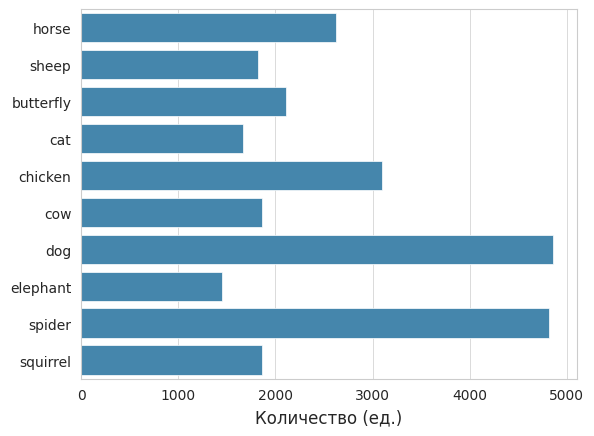
\includegraphics[width=0.8\textwidth]{images/class_dist.png}
    \caption{Распределение данных по классам}
    \label{fig:class_dist}
\end{figure}

\subsection{Архитектура AlexNet}
Архитектура AlexNet основана на идее постепенного уменьшения размера ядра сверток.
На первом сверточном слое используется ядра размера $11 \times 11$, затем ядро $5 \times 5$ и три свертки с ядром $3 \times 3$.
Большие ядра на первых сверточных слоях позволяют выделять большие объекты сразу.
Cхема модели представлена на рисунке \ref{fig:alexnet}.
\begin{figure}[h]
    \centering
    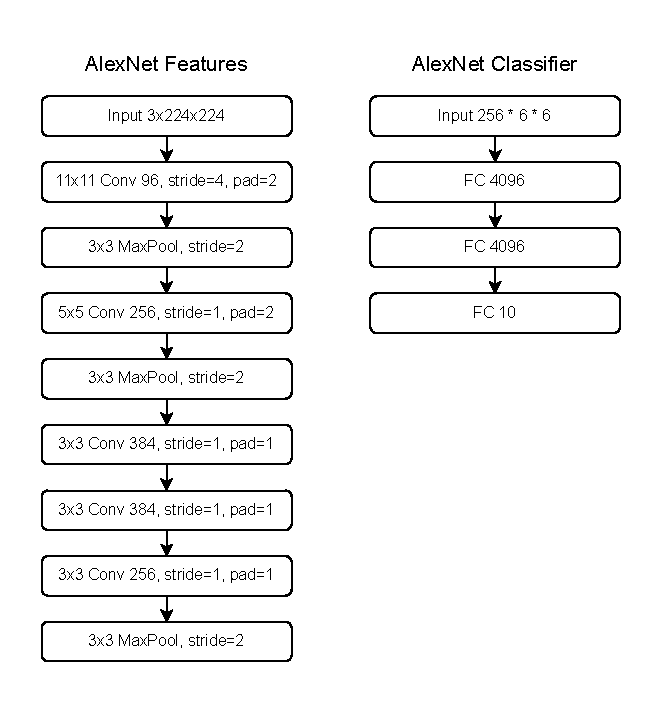
\includegraphics[width=0.8\textwidth]{images/alexnet_model.pdf}
    \caption{Схема архитектуры AlexNet}
    \label{fig:alexnet}
\end{figure}

В оригинальной модели AlexNet после первых двух сверточных слоев используется "local response" нормализация.
Помимо классической модели был реализован вариант с использованием более общего алгоритма "batch" нормализации.
В качестве оптимизатора обеих моделей использовался стохастический градиентный спуск с коэффициентом момента $0.9$ и размером batch равным 128.

Оригинальная модель показала лучший результат (на основе 10 запусков обучения) по сравнению с модификацией, которая использует batch нормализацию: $0.843$ против $0.83$ соответственно.
Результаты обучения моделей представлены на рисунках \ref{fig:alexnet_lrn} и \ref{fig:alexnet_bn}.
\begin{figure}[h]
    \centering
    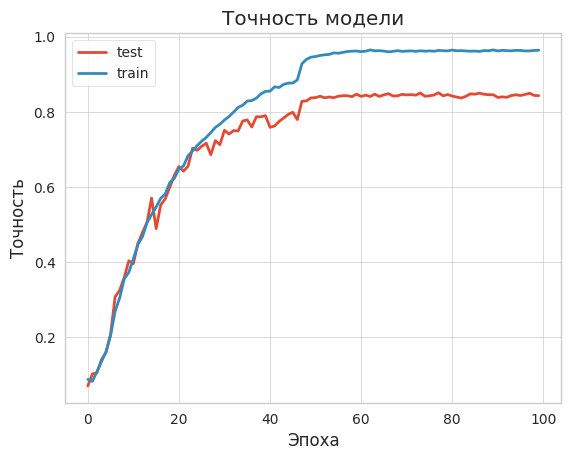
\includegraphics[width=0.65\textwidth]{images/alexnet_lrn_f1.png}
    \caption{График точности модели AlexNet с local response нормализацей}
    \label{fig:alexnet_lrn}
\end{figure}
\begin{figure}[h]
    \centering
    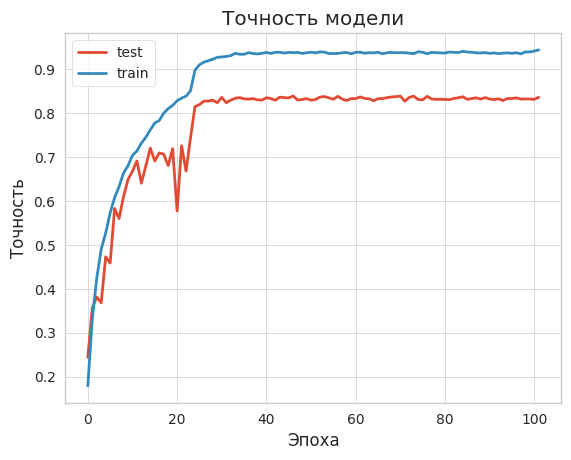
\includegraphics[width=0.65\textwidth]{images/alexnet_bn_f1.png}
    \caption{График точности модели AlexNet с batch нормализацей}
    \label{fig:alexnet_bn}
\end{figure}

Также к моделям был применен алгоритм визуализации Grad-CAM.
На рисункaх \ref{fig:alexnet_gradcam_1} и \ref{fig:alexnet_gradcam_2} представлен результат работы алгоритма для последнего сверточного слоя варианта с local response нормализацией.
\newpage
\begin{figure}[h]
    \centering
    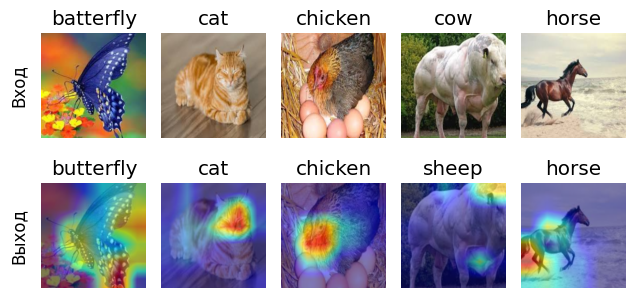
\includegraphics[width=0.8\textwidth]{images/alexnet_out_1.png}
    \caption{Тепловые карты Grad-CAM для модели AlexNet}
    \label{fig:alexnet_gradcam_1}
\end{figure}
\begin{figure}[h]
    \centering
    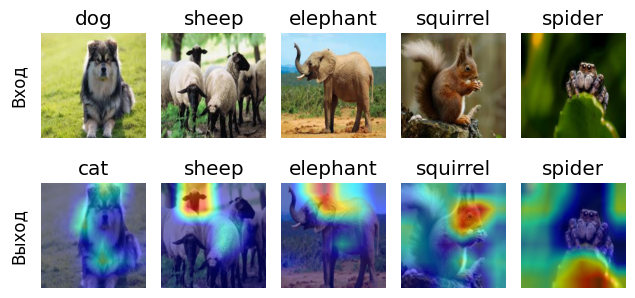
\includegraphics[width=0.8\textwidth]{images/alexnet_out_2.png}
    \caption{Тепловые карты Grad-CAM для модели AlexNet (продолжение)}
    \label{fig:alexnet_gradcam_2}
\end{figure}

Используя Grad-CAM можно сделать некоторые выводы о признаках, которые "выучила" модель.
Например, класс бабочки определяют ее крылья, класс лошади -- ее задние ноги и хвост, а класс паука предсказывается не по самому пауку, а по его окружению.
Последняя ситуация крайне вредна для модели, потому что схожий фон может быть у изображений и других животных.
Без алгоритма визуализации такое поведение модели предсказать было бы очень сложно.

В листинге \ref{listing:alexnet} приложения представлена програмная реализация архитектуры AlexNet.

\newpage
\subsection{Архитектура VGGNet}

В отличие от AlexNet, архитектура VGG не использует большие ядра сверток.
Вместо этого, используется больше слоев с малыми ядрами размера $3 \times 3$.
Такой подход имеет ряд преимуществ \cite{vggnet}. Во первых, несколько слоев с малыми свертками имееют намного меньше параметров: на один канал сверточного слоя со сверткой $121 \times 121$ необходимо 121 параметров, в то время как для 3 сверточных слоев необходимо всего $9 + 9 + 9 = 27$ параметров.
Во вторых, рецептивное поле 3 малого сверточного слоя имеет размер $3 + 2 + 2 = 7$ клеток, что соотвествует рецептивному полю сверточного слоя с ядром $7 \times 7$, имеющее большее число параметров.

Глубокие сети также выделяют более сложные признаки, качественно отличающиеся от признаков "широких" сетей вроде AlexNet, что будет продемонстрировано позже.

VGG на самом деле являются целым семейством моделей, поскольку единообразная организация сверточных слоев позволяет строить похожие модели разной глубины и ширины.
На рисунке \ref{fig:vgg13} изображена модель VGG13 (10 сверточных + 3 полносвязных слоя).
\begin{figure}[h]
    \centering
    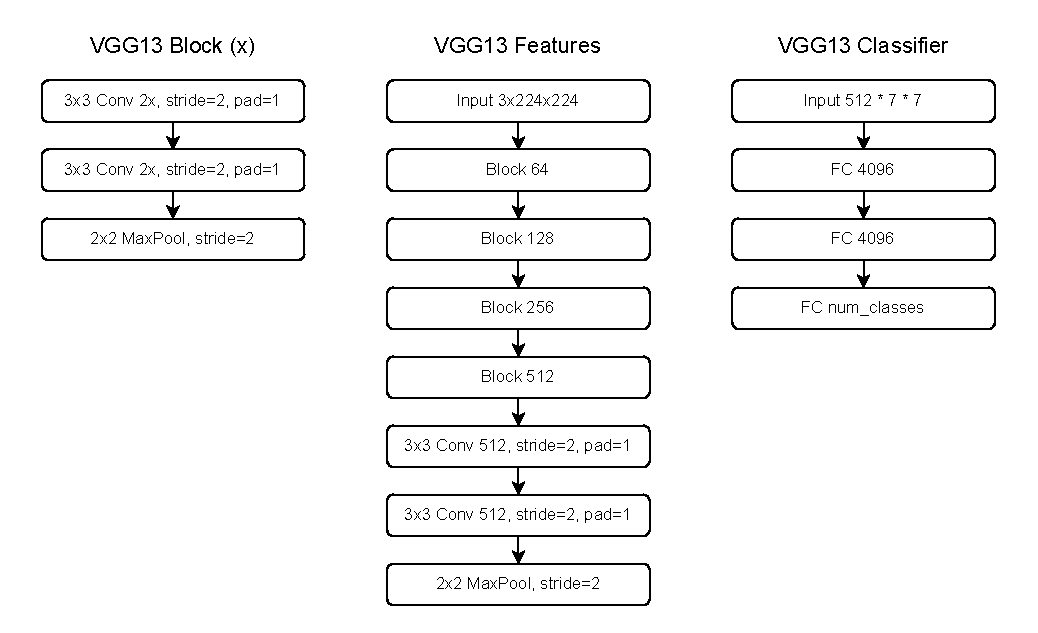
\includegraphics[width=0.8\textwidth]{images/vgg13_model.pdf}
    \caption{Модель VGG13}
    \label{fig:vgg13}
\end{figure}

Для рассматриваемого датасета предложена модификация модели VGG13.
В отличие от оригинала, модификация CVGG13 использует меньшее число параметров полносвязных слоев, а также использует batch нормализацию на каждом сверточном слое.
Меньший размер полносвязных слоев обусловлен малым размером тренировочных данных, на которых крупная модель (оригинальная VGG13 имеет порядка 130 млн. параметров) не сможет корректно обучиться.
Схема модифицированной модели представлена на рисунке \ref{fig:cvgg13}.
\begin{figure}[h]
    \centering
    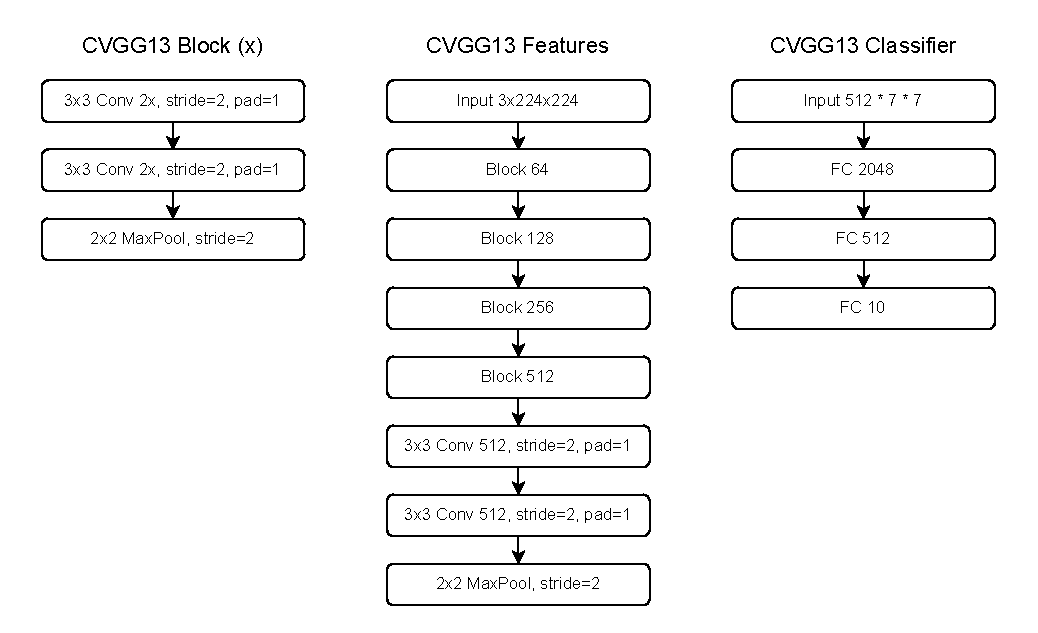
\includegraphics[width=0.8\textwidth]{images/cvgg13_model.pdf}
    \caption{Модель CVGG13}
    \label{fig:cvgg13}
\end{figure}

Для обучения CVGG13 использовался стохастический градиентный спуск с коэффициентом момента 0.9 и batch размера 64.
Модель получила отличные результаты как в точности, равной 0.915, так и в интерпретируемости признаков с помощью Grad-CAM.
Результаты обучения представлены на рисунке \ref{fig:cvgg13_f1}.
\newpage
\begin{figure}[h]
    \centering
    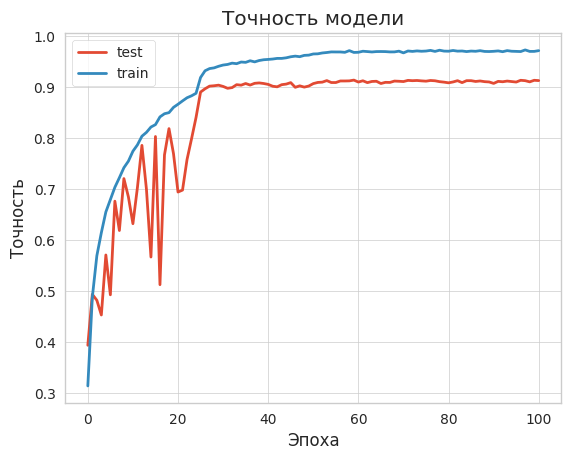
\includegraphics[width=0.8\textwidth]{images/cvgg13_f1.png}
    \caption{График изменения точности CVGG13}
    \label{fig:cvgg13_f1}
\end{figure}

Результаты применения Grad-CAM к последнему слою разработанной модели представлены на рисунках \ref{fig:cvgg13_gradcam_1} и \ref{fig:cvgg13_gradcam_2}.
\begin{figure}[h]
    \centering
    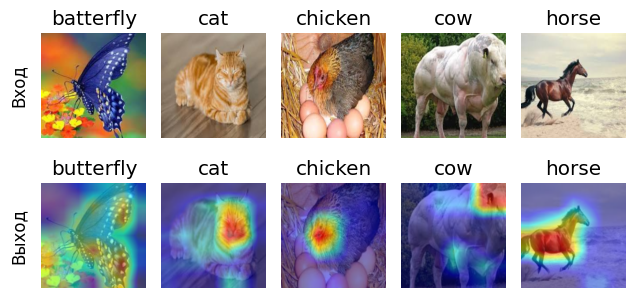
\includegraphics[width=0.85\textwidth]{images/cvgg13_out_1.png}
    \caption{Тепловые карты Grad-CAM для модели CVGG13}
    \label{fig:cvgg13_gradcam_1}
\end{figure}
\newpage
\begin{figure}[h]
    \centering
    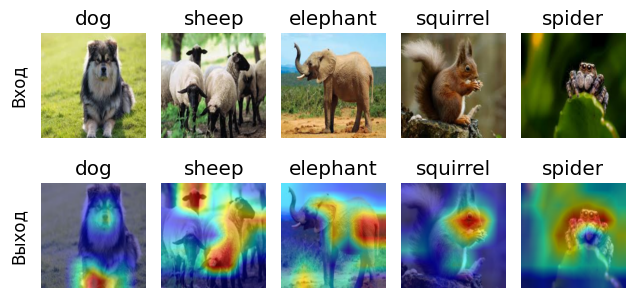
\includegraphics[width=0.85\textwidth]{images/cvgg13_out_2.png}
    \caption{Тепловые карты Grad-CAM для модели CVGG13 (продолжение)}
    \label{fig:cvgg13_gradcam_2}
\end{figure}

Изученные моделью признаки намного "крепче", чем признаки модели AlexNet.
В отличие от последней, класс паука определяется по самому пауку, а не его окружению.
Данная модель также показала более качественные тепловые карты и для остальных классов, особенно овцы и собаки.

Програмная реализация моделей семейства VGG13 представлена в листинге \ref{listing:vgg} приложения A.